\documentclass[12pt]{article}
\usepackage[english]{babel}
\usepackage[section]{placeins}
\usepackage{graphicx}
\usepackage{float}
	\begin{document}
		\begin{titlepage}

			\newcommand{\HRule}{\rule{\linewidth}{0.5mm}}
			\center
			
			\textsc{\LARGE Cardiff University}\\[1.5cm]
			\textsc{\Large CM3105 Security and Forensics}\\[0.5cm]

			\HRule \\[0.4cm]
				{ \huge \bfseries Computer Forensics Assignment 2013 - Technical Report}\\[0.4cm]
			\HRule \\[1.5cm]

			\begin{minipage}{0.4\textwidth}
				\begin{flushleft} \large
					\emph{Student Name:}\\
						Geraint \textsc{Harries} \newline
					\emph{Student Number:}\\
						1100682
				\end{flushleft}
			\end{minipage}
			~
			\begin{minipage}{0.4\textwidth}
				\begin{flushright} \large
					\emph{Lecturer(s):}\\
						Mike \textsc{Daley}
				\end{flushright}
			\end{minipage}\\[4cm]

			{\large \today}\\[3cm]

			\vfill

		\end{titlepage}

		\section{Abstract}

			\subsection{Tasking}

				For this assignment, we were tasked to analyse a USB image for evidence indicating the individual has been involved in industrial espionage against DataLog INc..

			\subsection{Executive Summary}
			
				This report will show evidence to suggest that Mona Simpson was involved with industrial espionage. Her role within DataLog Inc. allowed her to access information and supply it to \textit{'Ned'} (surname unknown).	

		\section{Preperation}
			\subsection{File Integrity}
				I was given an image of the USB entitled ‘fishytails.dd’. The first thing I did was make a MD5 and an SHA hash of the image.\newline\newline \textit{MD5 Hash Value: 2cea312fd83da54140717a4830fb33bf\newline SHA Hash Value: 54289cb3bfb8666d4d1836dd05ab74a13f1c8e19}\newline\newline I make a copy of the image and named it ‘fishytails.dd’. I ran the hash functions on this to verify the copy had been totally successful. I then made the copy read only by running the command.\newline\newline \textit{chmod 400 fishtailscopy.dd} \newline\newline I then verified it by listing the directory permissions using the ls - l command. This gave the following output:\newline\newline \textit{-r-------- 1 forensic forensic 473563136 Nov 22 20:09 fishytailscopy.dd} \newline\newline This allows me to investigate the data without touching the original image, thus eliminating the possibility of contamination.

			\subsection{Autopsy}
		
				I created a new case in autopsy, entitled ‘DataLogIncInvestigation’. I then added a new host, entitled ‘MonaSimpsonUSB’. I added the ‘fishytailscopy.dd’ to the case as a partition. I then verified the hash to check data integrity.	

		\section{Investigation}

			\subsection{Creating a Timeline}
				
				Using autopsy, I created a timeline. I did not enter a starting or end date (See Appendix 8.3, Figures 1,2,3 and 4 for full timeline table). You can see from the table that the creation date for all the files and directories is 1970, whereas the modification and access date is 2012. This suggests that the system clock of the original  directory and filelocation have been tampered with.\footnote{This could also be an unwanted remnant of creating the USB image for this coursework.}\newline\newline From the timeline, we can see several file and directory names. This will help us build a dirty word list (See Appendix 8.1)   

			\subsection{Media Analysis}

				Using the File Analysis tool within Aytopsy, I was able to step through the directories of the image and see all the files both present and deleted. Appendix 8.3, Figure 5, shows the directory structure of the USB image. \newline\newline In the directory \textit{My Tank/Documents}, I found a file called \textit{Shopping List.xls}. Although the \textit{.xls} suffix implies it is encoded with the Microsoft Excel File format, the metadata shown by autopsy shows that the file was originally created using Microsoft Office Word (See Appendix 8.3, Figure 6). I changed the suffix of the document to \textit{.doc}, Appendix 8.3, Figure 7 shows the documents as it was created. The message says 
				
				\begin{quotation}
					\noindent Hi, \newline I got it, its with angle fish, you know what to do, just run it through snake. \newline Ned 
				\end{quotation}

				\noindent \textit{Ned} is now someone we can identify as implicated. We can add the name \textit{Ned} to our dirty word list, as well as snake.\footnote{This answers part 1 of the basic requirements of the coursework. There is someone else implicated he is known as \textit{ned}}. A deleted file within the same directory \textit{\_i.xls}, also contains the message.  \newline\newline
				Within \textit{My Tanks/Documents/progs/for your eyes only/} there is a deleted python script called \_nake.py (See Appendix 8.3, Figure 8 and 9). Given the content of \textit{Shopping List.xls} when encoded with \textit{.doc} format, it's fair to assume that the deleted character is \textit{s}. This script takes the file \textit{combined.ppm}, decrypts it and returns the file \textit{decrypted.ppm}. This suggests that that an image \textit{combined.ppm} exists and that it contains secret content.\newline\newline

				\noindent In \textit{My Tank/Marines/My new Aquarium/new fish/} there are 4 images, three of which is deleted. The files are called, \textit{\_ombined.png, \_ombined.ppm, AngleFish.png, AngleFish.ppm}. It is fair to assume the missing characters of the first two files are c. \textit{combined.ppm} is the desired input for the script \textit{\_nake.py}. We can therefor assume that the script was intended to be used.\newline\newline

				\noindent I ran both \textit{.ppm} files through the \textit{\_nake.py} file. \textit{\_ombined.ppm} was unable to be decrypted however, \textit{AngleFish.ppm} was able to be and generated an image (See Appendix 8.3, Figure 11). The image \textit{AngleFish.ppm} uses stegonography which means that one file can be contained within another. This is what has been done here. The generated image in Appendix 8.3, Figure 11, is what was hidden within \textit{AngleFish.ppm}.\newline
				There are many other images of fish on the drive however I found no evidence to suggest that any steganographic techniques were used. I investigated these files however found no evidence to suggest they were worth reporting.

			\section{String Search}

				For the string search, I searched all the terms in the dirty words list (See Appendix 8.1). I searched the terms in the dirty word list without case sensitivity and showing the terms in ascii and unicode. I did not do a grep regular expression search. The results for the string search of the terms \textit{Angle, Fish, Ned} and \textit{Snake} are shown in Appendix 8.3 figures 19, 20, 21 and 22 respectively. The results did not show us anything that we hadn't seen before. 

			\section{Evidence}
				\subsection{Shopping List.xls}	
					\begin{tabular}{ l | p{8cm} }
						Evidence Number & 001  \\
			    			File Name & Shopping List.xls  \\
			      			File Path & C:/My Tank/Documents/  \\
						Date/ Time Created & Sun April 14 21:53:58 2013\\
						Created Using & Microsoft Office Word\\
						Additional Information & n/a \\
						Summary & A file encoded using Microsoft Office Word but displayed with Microsoft Office Excel\\
						MD5 Hash & 03c633e3ae39bfd27a59c2e2041eebd4\\
						Figure Reference & Appendix 8.3, Figure 7 and 12\\
					\end{tabular}
				\subsection{\_nake.py}
					\begin{tabular}{l | p{8cm}}
						Evidence Number & 002  \\
			    			File Name & \_nake.py  \\
			      			File Path & C:/My Tank/Documents/progs/  \\
						Date/ Time Created & Sun April 14 21:53:58 2013\\
						Created Using & Unkown\\
						Additional Information & It had been deleted\\
						Summary & A python script which decrpts an image using steganographic techniques\\
						MD5 Hash & 6fc0ed465f263bf06a10894b7a9a13\\
						Figure Reference & Appendix 8.3, Figure 8 and 9\\
					\end{tabular}

				\subsection{AngleFish.ppm}
					\begin{tabular}{l | p{8cm}}
						Evidence Number & 003  \\
			    			File Name & AngleFish.ppm \\
			      			File Path & C:/My Tank/Marines/My new Aquarium/  \\
						Date/ Time Created & Sun April 17 11:49:47 2013 \\
						Created Using & Unkown \\
						Additional Information & n/a \\
						Summary & Image of two fish\\
						MD5 Hash & 75f051e14ef0ed7c19cf4c04ab13d174 \\
						Figure Reference & Appendix 8.3, Figure 13\\
					\end{tabular}

				\subsection{decrypt.ppm}
					\begin{tabular}{l | p{8cm}}
						Evidence Number & 004  \\
			    			File Name & decrypt.ppm \\
			      			File Path & \\
						Date/ Time Created & \\
						Created Using & \_nake.py \\
						Additional Information & This image was generated on my machine. It was embedded within the image AngleFish.ppm using steganography.\\
						Summary & An image containing a phone attached to a circuit board \\
						MD5 Hash & 01bd7e725008c55f60e999e9add4149d \\
						Figure Reference & Appendix 8.3, Figure 11\\
					\end{tabular}

				\subsection{combined.ppm}
					\begin{tabular}{l | p{8cm}}
						Evidence Number & 005  \\
			    			File Name & combined.ppm \\
			      			File Path & C:/Nothing Here to see/New folder/New folder/new fish/New folder/\\
						Date/ Time Created & Sun April 14 21:53:59 2013\\
						Created Using & Unknown \\
						Additional Information & This image uses steganography to hide the image decrypt.ppm\\
						Summary & Image of two fish\\
						MD5 Hash & 75f051e14ef0ed7c19cf4c04ab13d174 \\
						Figure Reference & Appendix 8.3, Figure 14\\
					\end{tabular}
					
				\subsection{\_i.xls}
					\begin{tabular}{l | p{8cm}}
						Evidence Number & 006  \\
			    			File Name & \_i.xls \\
			      			File Path & C:/My Tank/Documents/ \\
						Date/ Time Created & Sun Apr 14 21:53:58 \\
						Created Using & Unknown \\
						Additional Information & It has been deleted \\
						Summary & File containing text \\
						MD5 Hash & d231d480ebc0b06ef3c51094ca7c99d0 \\
						Figure Reference & Appendix 8.3, Figure 15\\
					\end{tabular}

				\subsection{Questions specifically asked}

					\subsubsection{Is there anyone else implicated?}
						In section 3.2, I highlight that \textit{Ned} (Surname unknown) is implicated.
					\subsubsection{Where is Penelope planning to travel to?}
						In the IP packets supplied by DataLog Inc. Mona is messaging someone. The message says:
						\begin{quotation}
							\noindent Here's the secret recipe. I just downloaded it from the file server. Just copy to a thumb drive and you're good to go :-). 
						\end{quotation}

						\noindent The person then replies

						\begin{quotation}
							\noindent See you in hawaii!
						\end{quotation}

						\noindent This implies that Mona will be travelling to Hawaii soon.
					\subsubsection{Can you find the stolen photo?}
						Section 3.2 explains how I found the stolen photo
					\subsubsection{How was the file hidden and how did you recover it?}
						Section 3.2 explains how the image was hidden.	
					\subsubsection{What other steps have been taken (if any) have been taken to hide evidence?}
						They have deleted several files, this is shown in section 6. They have also tried to hide files in the depths of sub folders. 	
			\section{Deleted Files}

				I used the \textit{All Deleted Files} function within Autopsy to find all the deleted files from the image.

				\subsection{\_i.xls}
					\begin{tabular}{l | p{8cm}}
						Evidence Number & 006  \\
			    			File Name & \_i.xls \\
			      			File Path & C:/My Tank/Documents/ \\
						Date/ Time Created & Sun Apr 14 21:53:58 \\
						Created Using & Unknown \\
						Additional Information & It has been deleted \\
						Summary & File containing text \\
						MD5 Hash & d231d480ebc0b06ef3c51094ca7c99d0 \\
						Figure Reference & Appendix 8.3, Figure 15\\
					\end{tabular}

				\subsection{\_nake.py}
					\begin{tabular}{l | p{8cm}}
						Evidence Number & 002  \\
			    			File Name & \_nake.py  \\
			      			File Path & C:/My Tank/Documents/progs/  \\
						Date/ Time Created & Sun Apr 14 21:53:58 2013\\
						Created Using & Unkown\\
						Additional Information & It had been deleted\\
						Summary & A python script which decrpts an image using steganographic techniques\\
						MD5 Hash & 6fc0ed465f263bf06a10894b7a9a13\\
						Figure Reference & Appendix 8.3, Figure 8 and 9\\
					\end{tabular}

				\subsection{\_ombined.png}
					\begin{tabular}{l | p{8cm}}
						Evidence Number & 007  \\
			    			File Name & \_ombined  \\
			      			File Path & C:/My Tank/Marines/My new Aquarium/new fish/Something fishy/  \\
						Date/ Time Created & Sun Apr 14 21:53:59 2013 \\
						Created Using & Unkown \\
						Additional Information & It had been deleted \\
						Summary & Image of two fish\\
						MD5 Hash & 0a1cb58285957988d523cc6eff08254f\\
						Figure Reference & Appendix 8.3, Figure 16\\
					\end{tabular}

				\subsection{AngleFish.png}
					\begin{tabular}{l | p{8cm}}
						Evidence Number & 008  \\
			    			File Name & AngleFish.png \\
			      			File Path & C:/My Tank/Marines/My new Aquarium/new fish/Something fishy  \\
						Date/ Time Created & Sun April 14 21:53:59 2013 \\
						Created Using & Unkown \\
						Additional Information & n/a \\
						Summary & Image of two fish\\
						MD5 Hash & 0a1cb58285957988d523cc6eff08254f \\
						Figure Reference & Appendix 8.3, Figure 17\\
					\end{tabular}
				
				\subsection{\_ombined.ppm}
					\begin{tabular}{l | p{8cm}}
						Evidence Number & 009  \\
			    			File Name & \_ombined.ppm \\
			      			File Path & C:/My Tank/Marines/My new Aquarium/new fish/Something Fishy/  \\
						Date/ Time Created & Sun Apr 17 11:49:47 2013 \\
						Created Using & Unkown \\
						Additional Information & n/a \\
						Summary & A series of numbers\\
						MD5 Hash & b6e0f5979181a3f46dfddacbf4de5b56 \\
						Figure Reference & Appendix 8.3, Figure 18\\
					\end{tabular}

		\section{Summary}

			I made a MD5 hash of the image after I had finished investigating.  \newline MD5 Hash: 2cea312fd83da54140717a4830fb33bf \newline This matches the first MD5 hash, meaning that the integrity of the image remains.\newline
			The evidence suggests that she was involved with industrial espionage as some images on the USB image use stegonography to hide evidence and many files have been deleted to hide information from law enforcement agencies.

		\section{Appendix}

			\subsection{Dirty Word List}

				\begin{itemize}
					\item Angle
					\item Fish
					\item Snake
					\item Ned
				\end{itemize}

			\subsection{Tools Used}

				\begin{itemize}
					\item Autopsy
					\item Vim
					\item Libre Office
				\end{itemize}

				Autopsy automated a lot of unix commands, it seemed the obvious choice for a quick analysis. Vim is a terminal text editor which I used to view some of the files in. Libre Office was useful to view \textit{Shopping List} in and viewing it with different suffixes.

			\subsection{Figures}
				
				\begin{figure}[ht!]
					\centering
					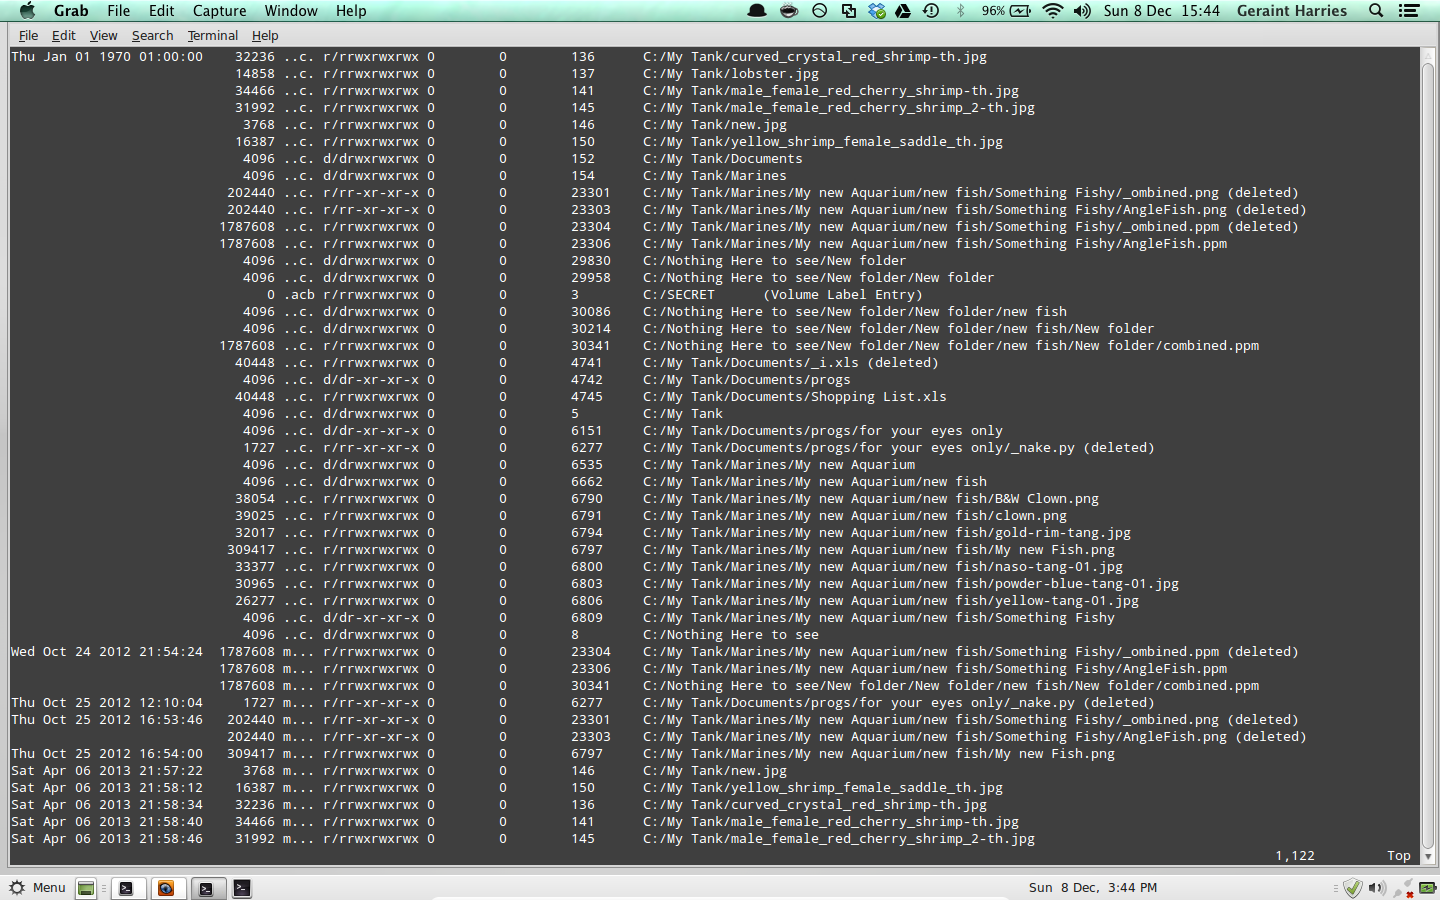
\includegraphics[width=12cm]{Images/TimeLine1.png}
					\caption{Timeline Page 1}
				\end{figure}
				\begin{figure}[ht!]
					\centering
					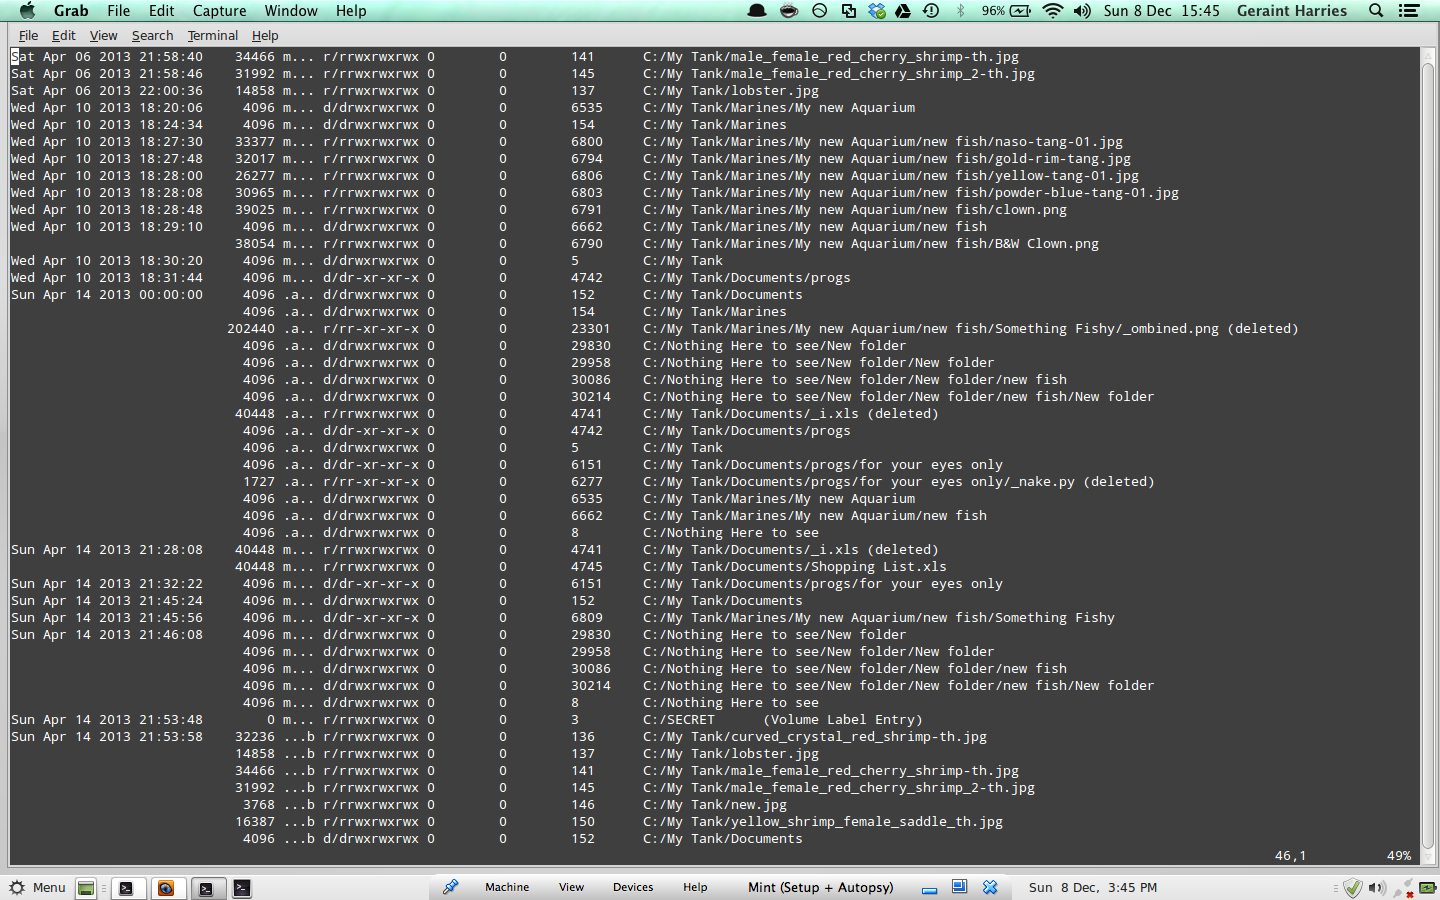
\includegraphics[width=12cm]{Images/TimeLine2.png}
					\caption{Timeline Page 2}
				\end{figure}
				\begin{figure}[ht!]
					\centering
					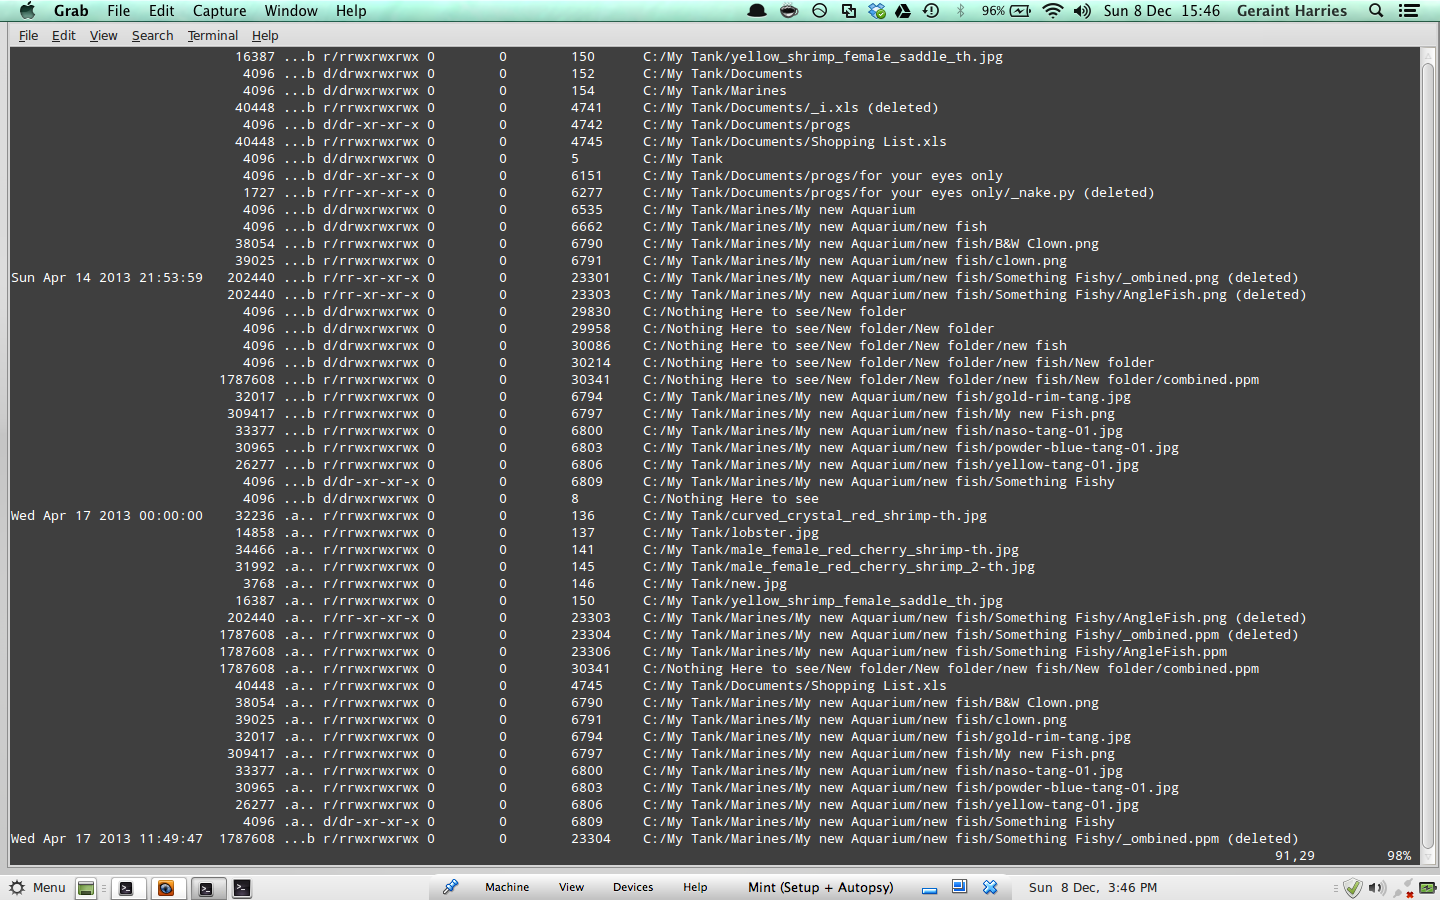
\includegraphics[width=12cm]{Images/TimeLine3.png}
					\caption{Timeline Page 3}
				\end{figure}
				\begin{figure}[ht!]
					\centering
					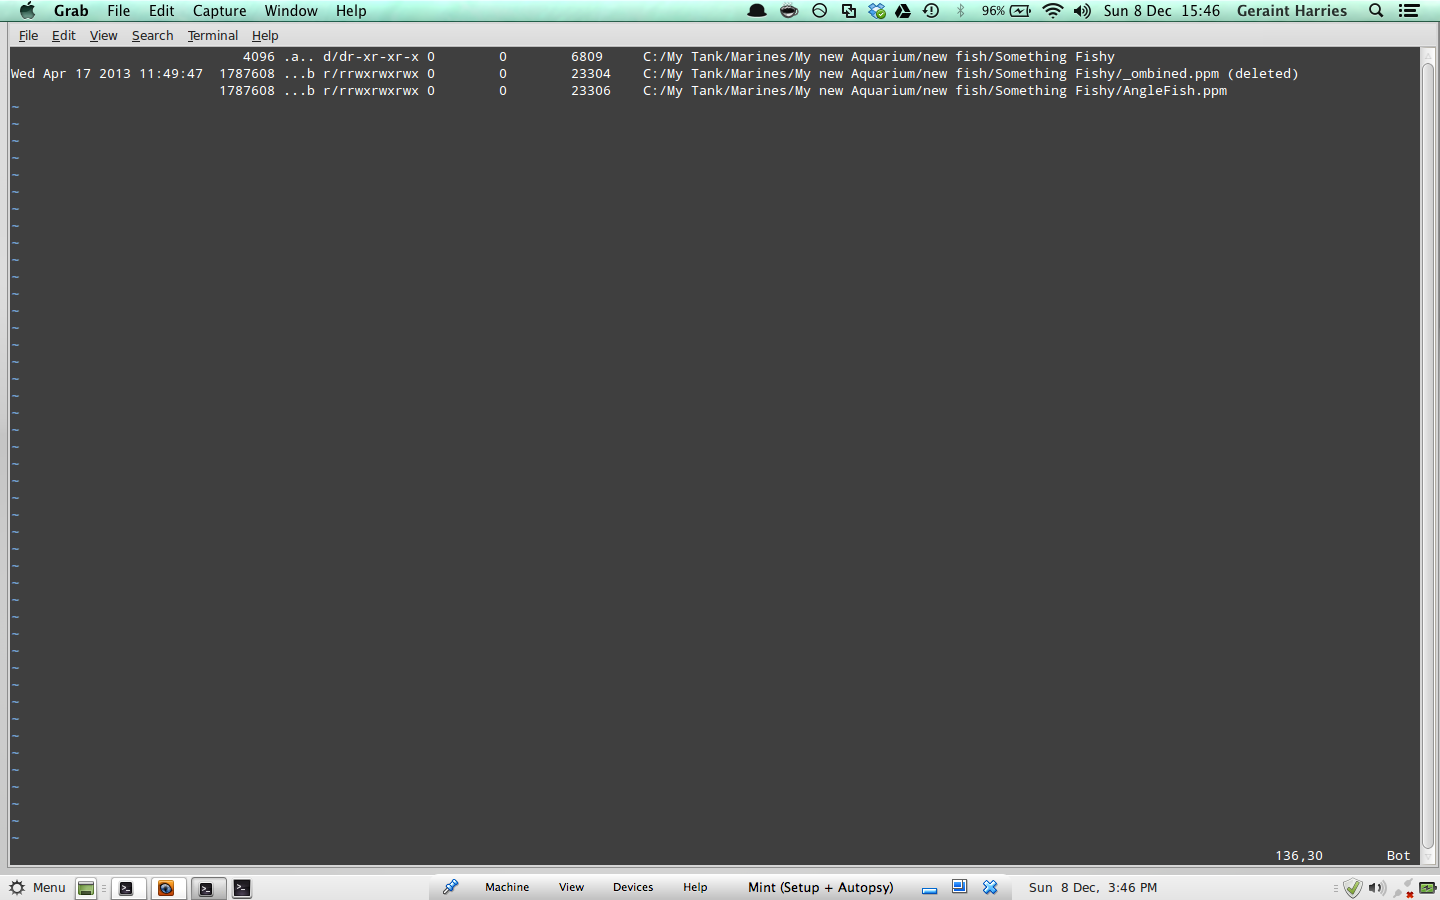
\includegraphics[width=12cm]{Images/TimeLine4.png}
					\caption{Timeline Page 4}
				\end{figure}

				\begin{figure}[ht!]
					\centering
					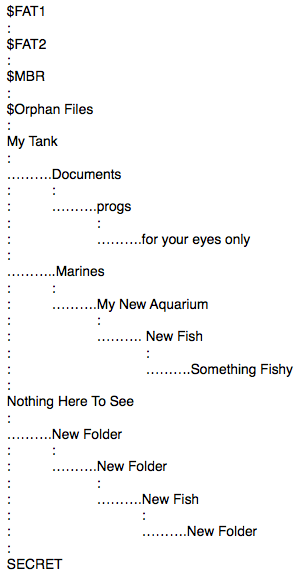
\includegraphics[width=5cm]{Images/DirectoryStructure.png}
					\caption{Directory Structure}
				\end{figure}
			
				\begin{figure}[ht!]
					\centering
					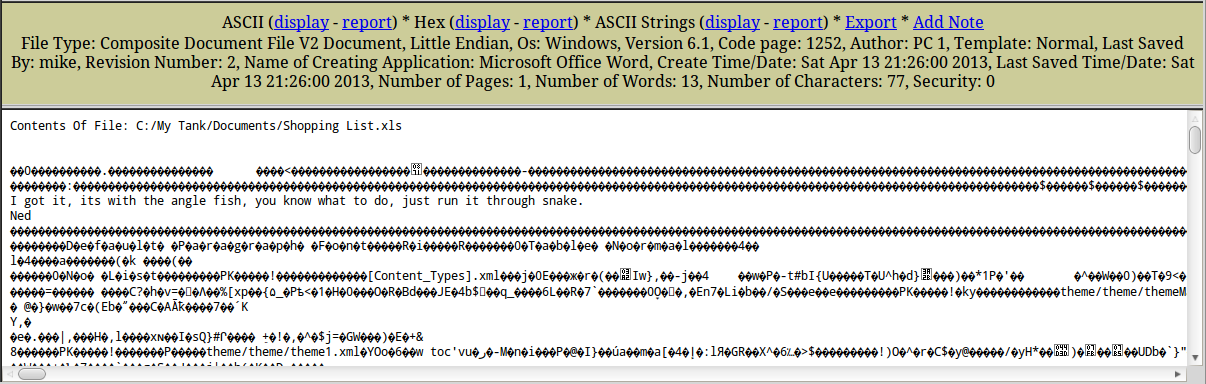
\includegraphics[width=\textwidth]{Images/WordExcel.png}
					\caption{Shopping List.xls contents and metadata}
				\end{figure}

				\begin{figure}[ht!]
					\centering
					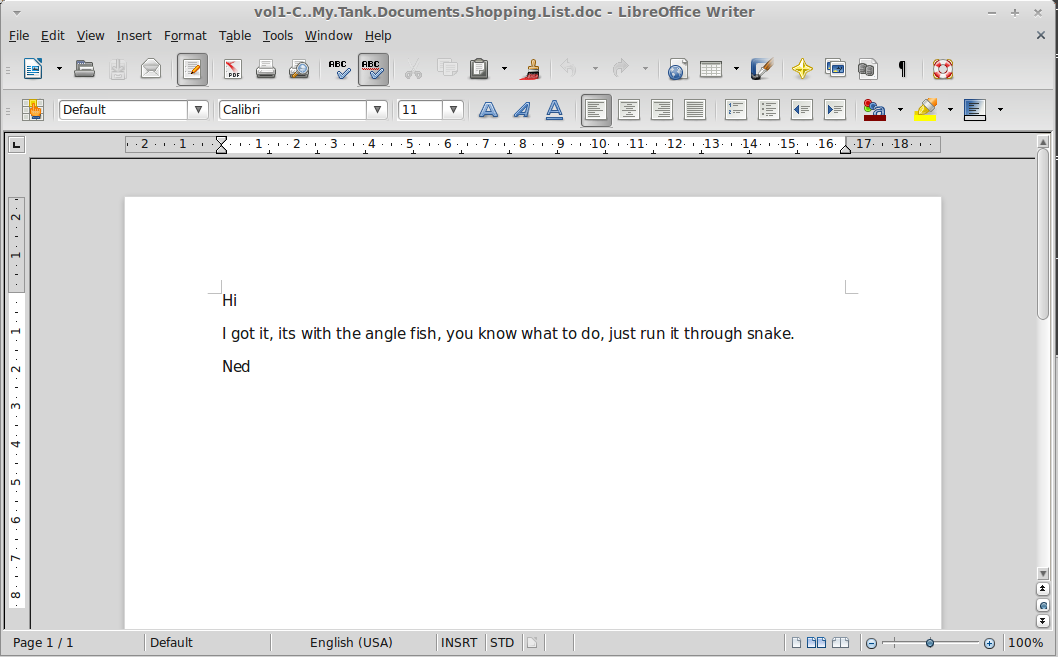
\includegraphics[width=12cm]{Images/ShoppingListWord.png}
					\caption{Shopping List.xls encoded as a .doc file}
				\end{figure}

				\begin{figure}[ht!]
					\centering
					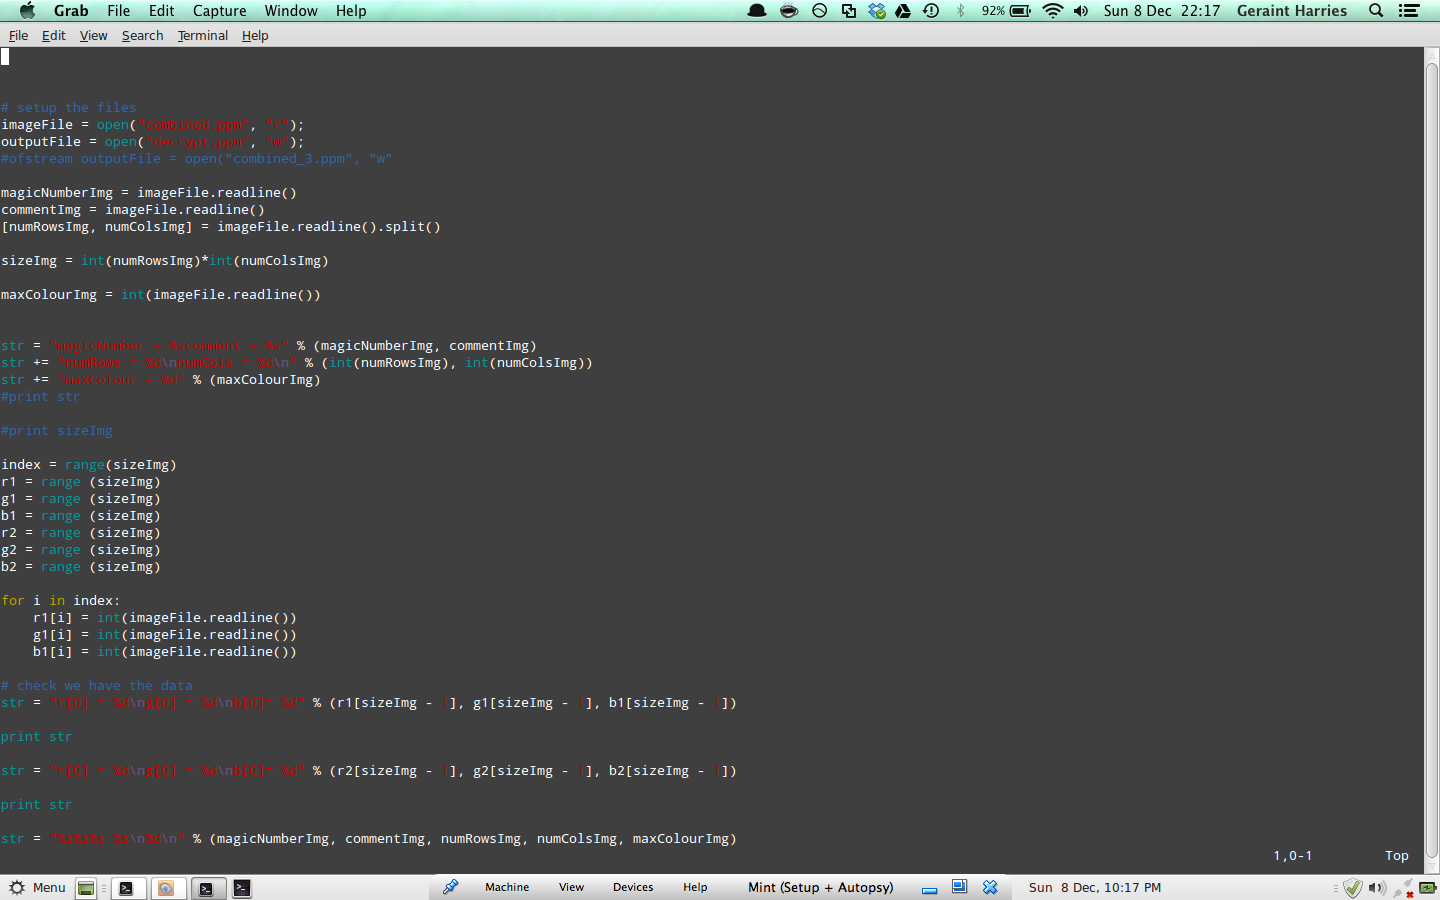
\includegraphics[width=12cm]{Images/_nape1.png}
					\caption{\_nake.py Page 1}
				\end{figure}

				\begin{figure}[ht!]
					\centering
					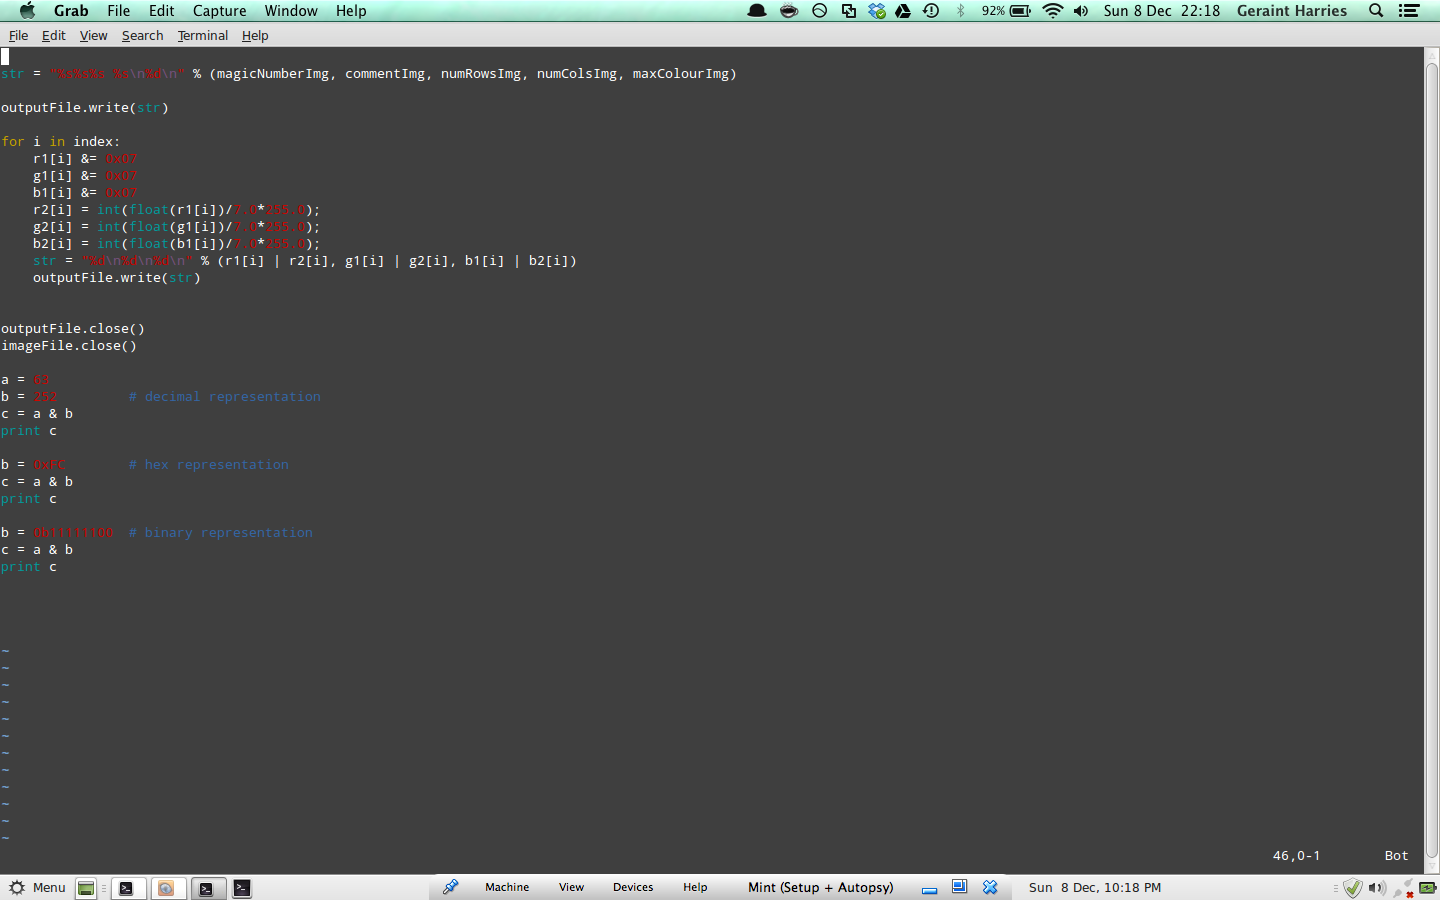
\includegraphics[width=12cm]{Images/_nape2.png}
					\caption{\_nake.py Page 2}
				\end{figure}
				
				\begin{figure}[ht!]
					\centering
					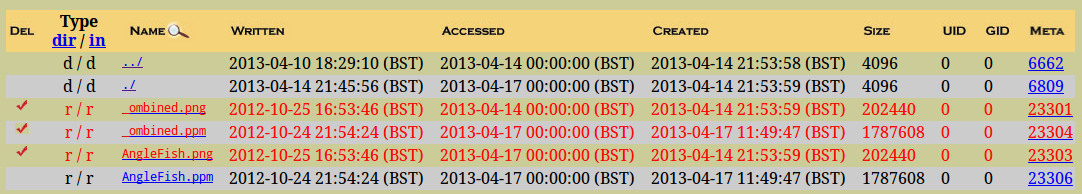
\includegraphics[width=10cm]{Images/4files.png}
					\caption{4 files, 3 of which are deleted}
				\end{figure}

				\begin{figure}[ht!]
					\centering
					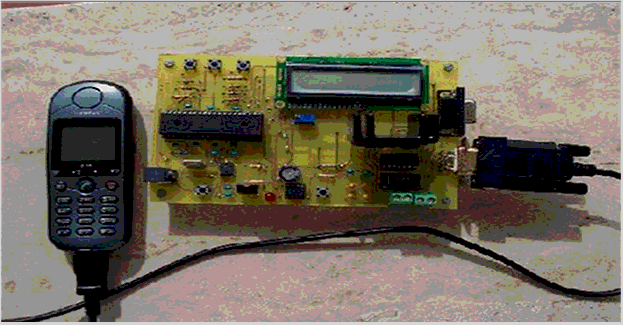
\includegraphics[width=12cm]{Images/decrypt.png}
					\caption{This image was generated by running AngleFish.ppm through the \_nake.py script}
				\end{figure}
				
				\begin{figure}[ht!]
					\centering
					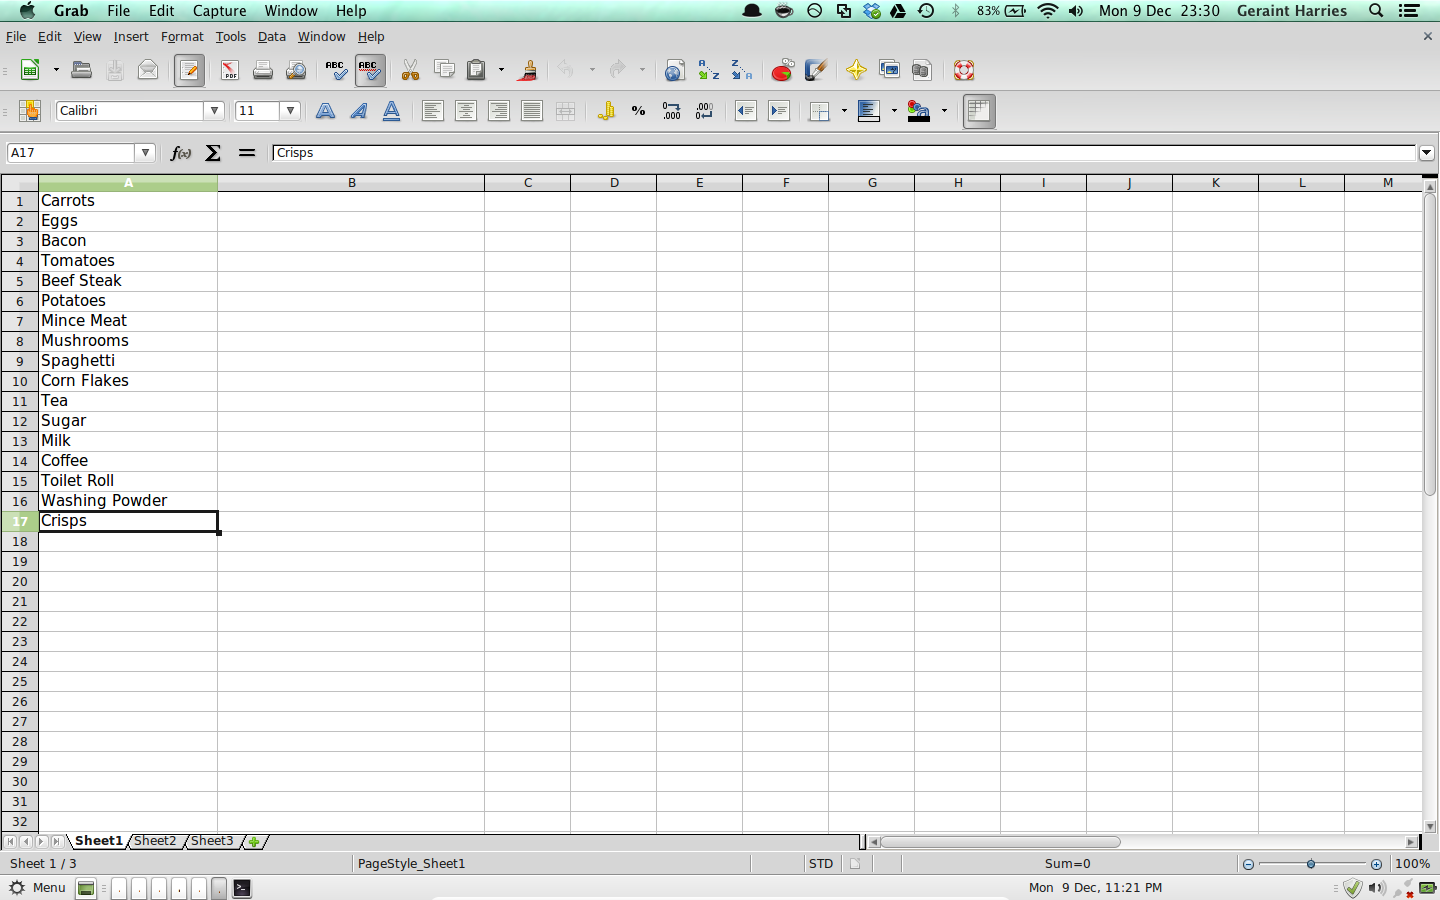
\includegraphics[width=12cm]{Images/ShoppingListExcel.png}
					\caption{Shopping List.xls encoded as a .xls file}
				\end{figure}
				
				\begin{figure}[ht!]
					\centering
					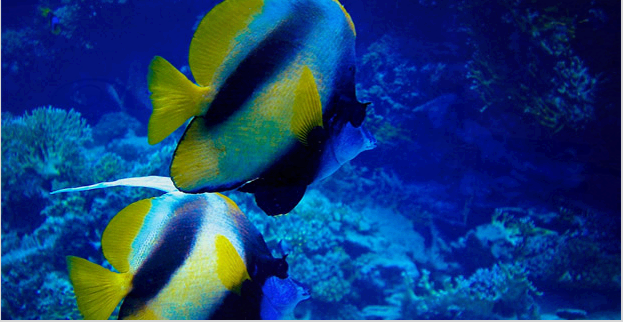
\includegraphics[width=12cm]{Images/AngleFishPpm.png}
					\caption{AngleFish.ppm}
				\end{figure}

				\begin{figure}[ht!]
					\centering
					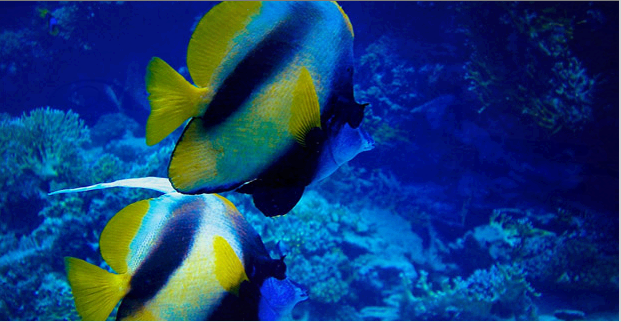
\includegraphics[width=12cm]{Images/CombinedPpm.png}
					\caption{Combined.ppm}
				\end{figure}
				
				\begin{figure}[ht!]
					\centering
					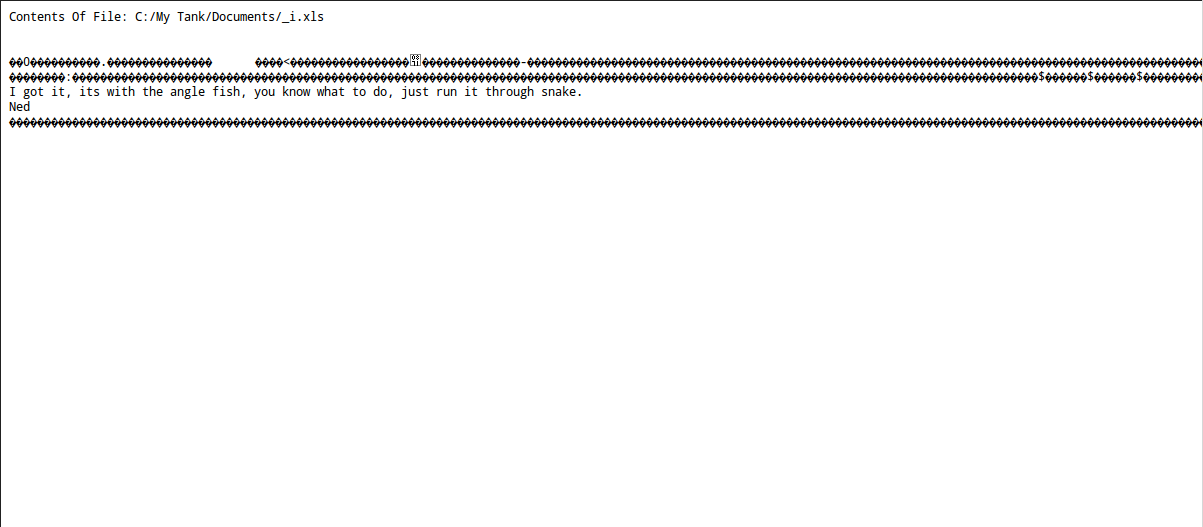
\includegraphics[width=12cm]{Images/_i.png}
					\caption{\_i.xls}
				\end{figure}

				\begin{figure}[ht!]
					\centering
					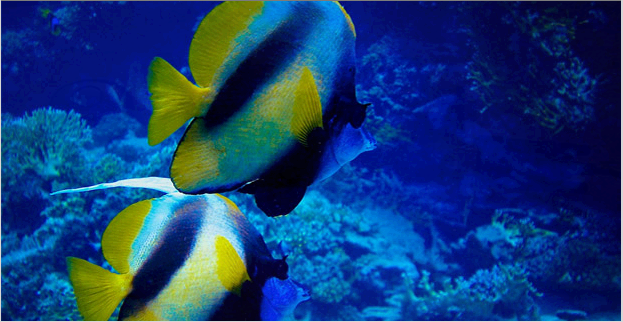
\includegraphics[width=12cm]{Images/_ombinedPng.png}
					\caption{\_ombined.png}
				\end{figure}

				\begin{figure}[ht!]
					\centering
					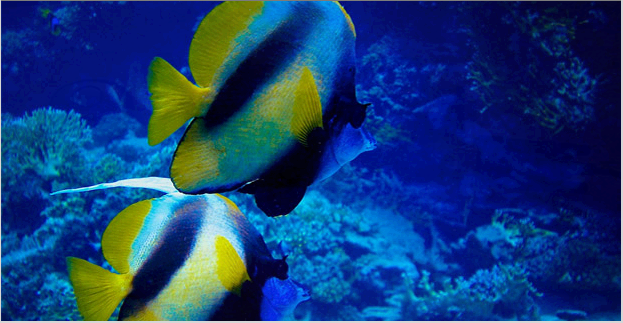
\includegraphics[width=12cm]{Images/AngleFishPng.png}
					\caption{AngleFish.png}
				\end{figure}

				\begin{figure}[ht!]
					\centering
					
\includegraphics[width=12cm]{Images/_ombinedPpm.png}
					\caption{\_ombined.ppm}
				\end{figure}

				\clearpage

				\begin{figure}[h]
					\centering
					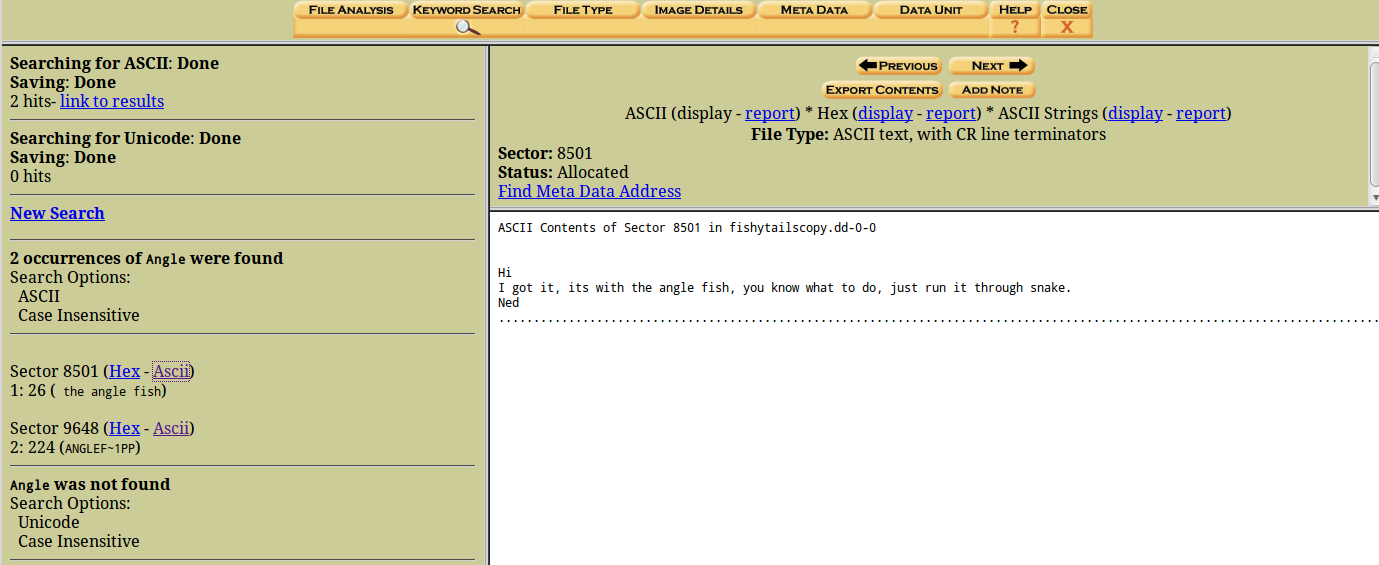
\includegraphics[width=12cm]{Images/AngleKeyWord.png}
					\caption{The keyword search results for searching the term \textit{Angle}}
				\end{figure}

				\begin{figure}[h]
					\centering
					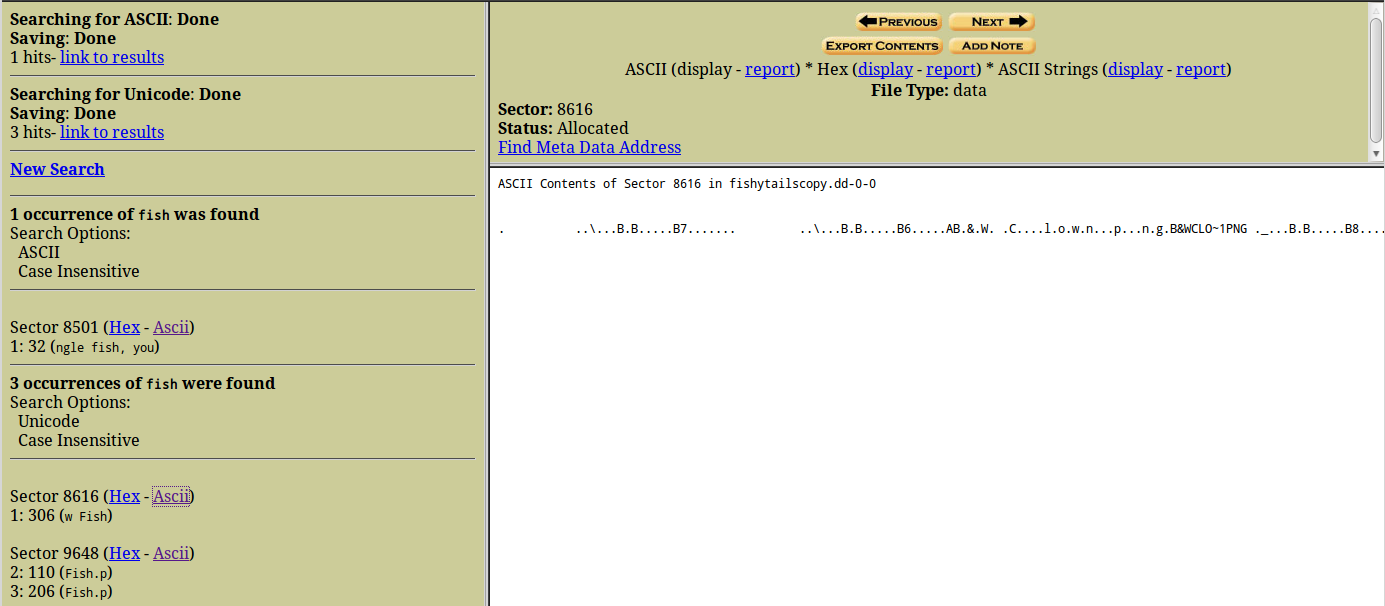
\includegraphics[width=12cm]{Images/FishKeyWord.png}
					\caption{The keyword search results for searching the term \textit{Fish}}
				\end{figure}

				\clearpage

				\begin{figure}[h]
					\centering
					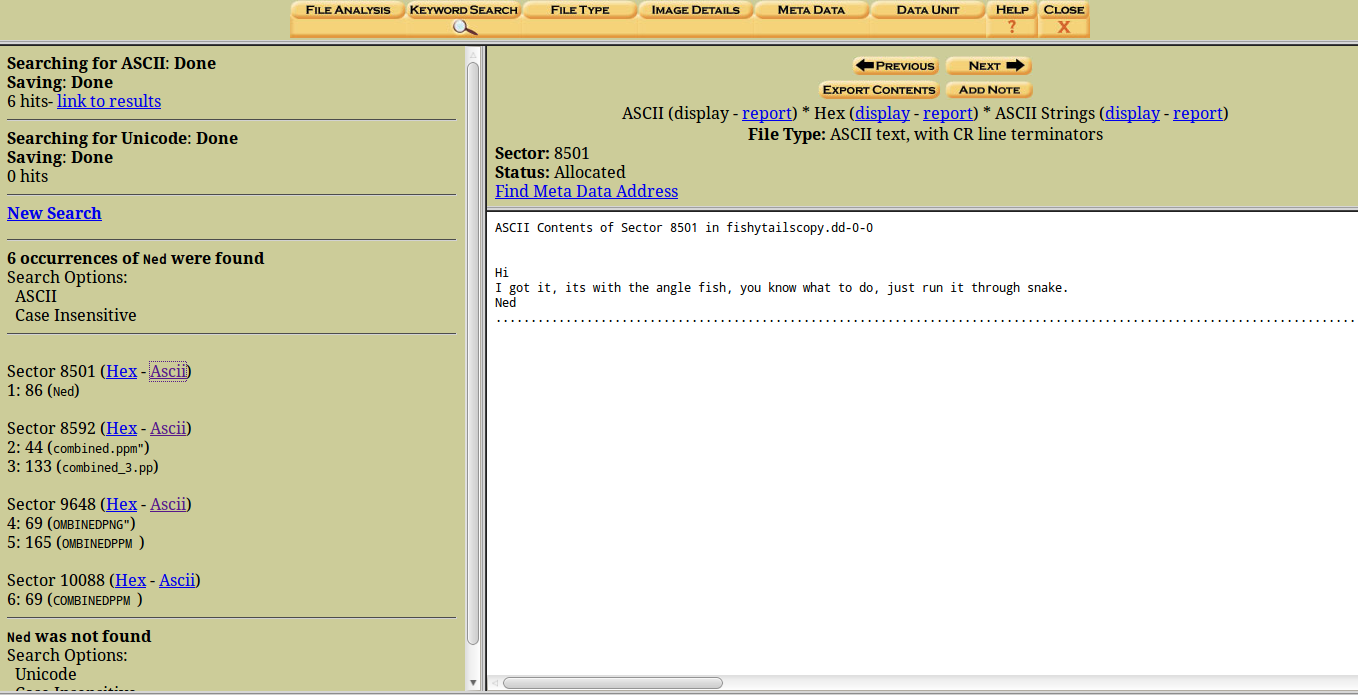
\includegraphics[width=12cm]{Images/NedKeyWord.png}
					\caption{The keyword search results for searching the term \textit{Ned}}
				\end{figure}	

				\begin{figure}[h]
					\centering
					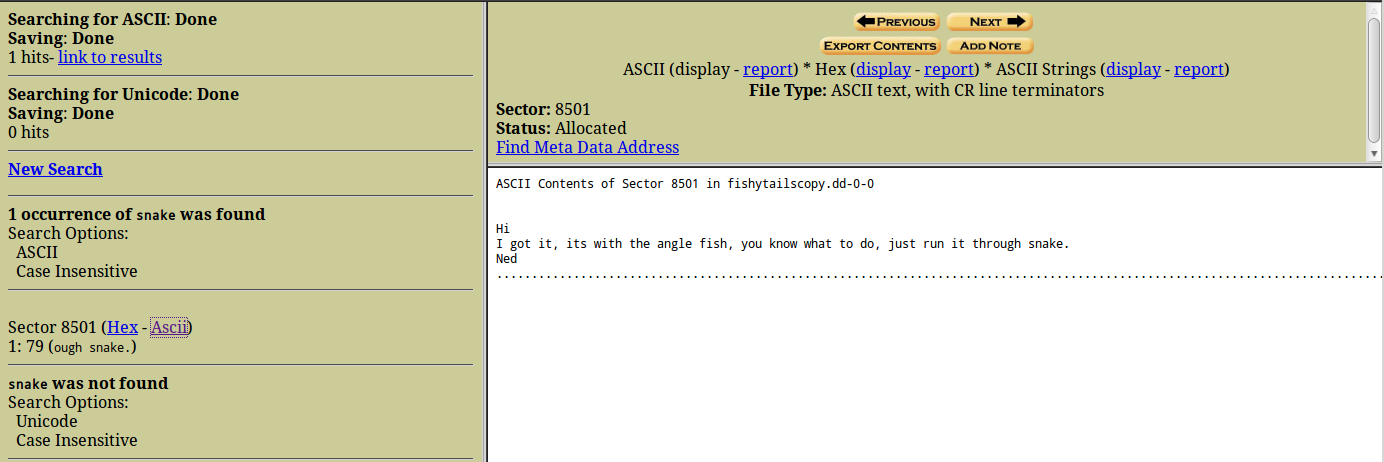
\includegraphics[width=12cm]{Images/SnakeKeyWord.png}
					\caption{The keyword search results for searching the term \textit{Snake}}
				\end{figure}

	\end{document}
